% chktex-file 46
%!TeX spellcheck = en-US,it-IT

\chapter{Cluster scalability}
In the thesis early stages, experiments have been done with the Distributed
Keras framework~\cite{distkeras} developed at CERN
but BigDL seemed more promising so we continued with this library.
Initially training was performed with a cluster formed of an $8$ cores master node and
$\SI{16}{\giga\byte}$ (\textit{xlarge}) and $5$ slaves with $2$ cores each
and $\SI{4}{\giga\byte}$ (\textit{medium}). Then it became clear
that, for the task, it was better an architecture with a \textit{medium} master and $5$
\textit{xlarge} slaves due to the fact that all the heavy lift is performed by workers.
On the GPU architecture side we had available an \textit{Nvidia Titan
 Xp}\footnote{https://www.nvidia.com/en-us/titan/titan-xp/} and an \textit{Nvidia RTX 2080
 FE}\footnote{https://www.nvidia.com/en-us/geforce/graphics-cards/rtx-2080/} graphics
cards.

We tested our model with several optimizers implemented by BigDL and Keras libraries.
The standard optimizer SGD, Adam\cite{Adam}, Adamax\cite{Adam}, Adadelta\cite{Adadelta}
and Adagrad\cite{Adagrad}. Cluster performance is evaluated between different numbers of
nodes and available GPUs. Results are shown in Fig.~\ref{1} and Fig.~\ref{2}.
\begin{figure}[H]
 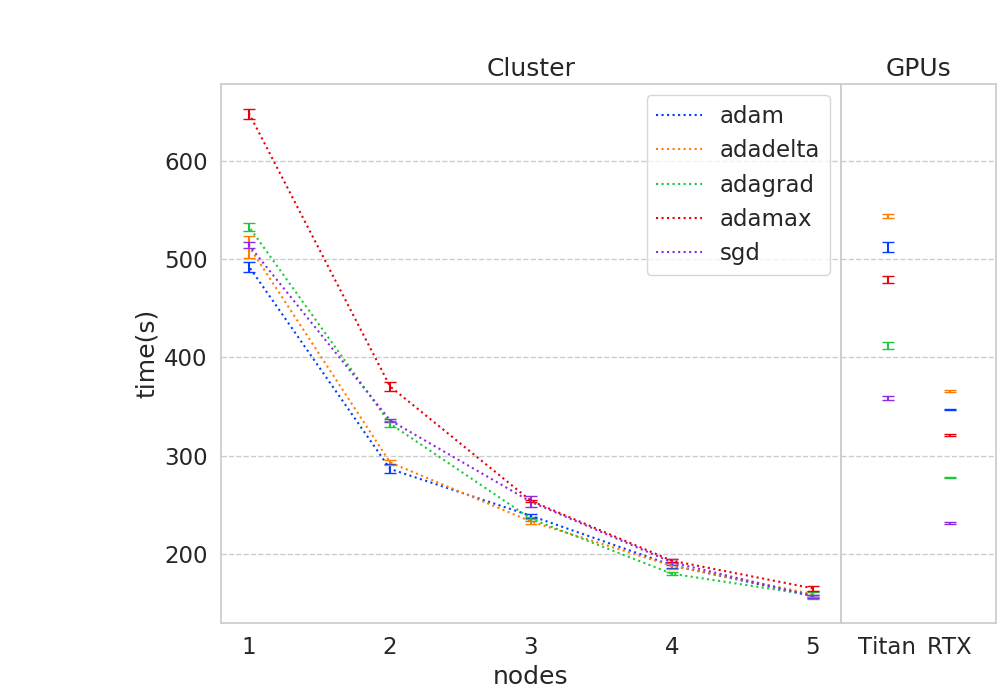
\includegraphics[scale=0.4]{figures/absolute.png}
 \caption{Number of nodes versus execution time for $1$ epoch}
 \label{1}
\end{figure}
\begin{figure}[H]
 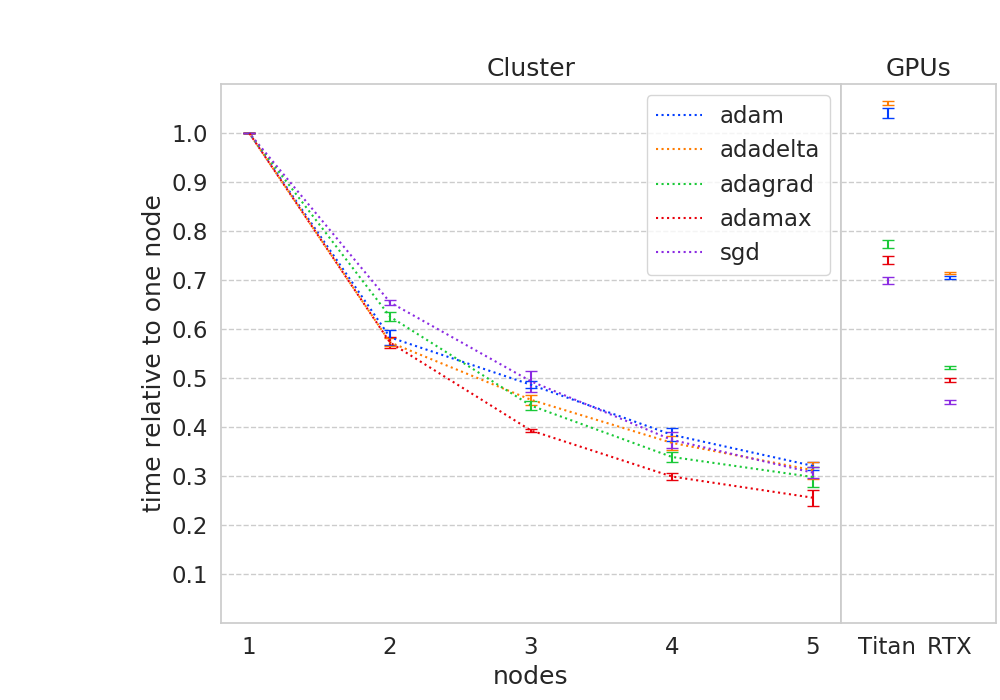
\includegraphics[scale=0.4]{figures/relative.png}
 \caption{Relative time regard execution with one node}
 \label{2}
\end{figure}

As shown in the Fig.~\ref{1} the performances improve by adding nodes, as intended. The
improvement is not linear, the difference in time performance between optimizers decrease
with increasing number of nodes. A simple interpretation could be that with more nodes
the training bottleneck is on the network side so the difference in time performance
between optimizers become less significant.
To support this hypothesis in Fig.~\ref{2} it can be seen that performance increase
approximately by $30\%$ - $40\%$ for each added node but relative improvement shrink
with the increment of the nodes. This may be due to the fact that the increase in the
number of nodes is limited by the time required for their communication with the
master.

The graphs also show that latest \textit{Nvidia} consumer-grade GPUs have comparable
performance with multi-cores CPUs.
Remembering that every node has $8$ it can be seen that in this test the \textit{Titan Xp}
can compete with an $8$ - $16$ cores cluster, depending on the chosen optimizer.
The \textit{rtx 2080} gets better results and is comparable with the performance of a $16$ -
$32$ cores cluster. This difference could be related to the different GPUs
\textit{Pascal}~\cite{pascal} and \textit{Turing}~\cite{turing} architectures. It could
be also noted that in this case the performances are strongly influenced by the chosen
optimizer. Not easily explainable this aspect should be further explored.
